%%%%%%%%%%%%%%%%%%%%%%%%%%%%%%%%%%%%%%%%%%%%%%%%%%%%%%%%%%%%%%%%%%%%%%%%%%%%%%%%%%%%%
%																					%
%	TRABAJO: Paper Redes de Petri Temporizadas										%
%																					%
%		Titulo: 	IP cores para la Ejecucion de Redes de Petri Temporales en FPGA	%
%																					%
%		Autores:	Julian Nonino													%
%					Carlos Renzo Pisetta											%
%					Orlando Micolini												%
%																					%
%	Seccion: Documento principal													%	
%	Archivo: 1_redes_petri_temporizadas.tex											%
%																					%
%%%%%%%%%%%%%%%%%%%%%%%%%%%%%%%%%%%%%%%%%%%%%%%%%%%%%%%%%%%%%%%%%%%%%%%%%%%%%%%%%%%%%
%	REVISIONES																		%
%																					%
%		17/10/2012																	%
%			Julian Nonino															%
%				Creacion de este archivo en base al template de Michael Shell		%
%													bare_jrnl.tex					%
%													V1.3							%
%													2007/01/11						%
%													by Michael Shell				%
%													http://www.michaelshell.org/	%
%				Este archivo utiliza la clase IEEEtrans.cls version 1.7 o posterior	%
%				Siendo el tipo de documento 'journal'								%
%																					%
%		18/10/2012																	%
%			Julian Nonino															%
%				Division del trabajo en distintos archivos e inclusion de los		%
%				mismos dentro de este archivo para que sea el documento principal	%
%				del trabajo.														%
%		18/10/2012																	%
%			Renzo Pisetta															%
%				Agregadas tres referencias											%
%		22/10/2012																	%
%			Julian Nonino															%
%				Nueva bibliografia con el formato de IEEE							%
%		04/04/2013																	%
%			Renzo Pisetta															%
%				Agregadas include redes de tiempo temporales						%
%																					%
%%%%%%%%%%%%%%%%%%%%%%%%%%%%%%%%%%%%%%%%%%%%%%%%%%%%%%%%%%%%%%%%%%%%%%%%%%%%%%%%%%%%%

% Also note that the "draftcls" or "draftclsnofoot", not "draft", option
% should be used if it is desired that the figures are to be displayed in
% draft mode.

\documentclass[journal]{IEEEtran}
% If IEEEtran.cls has not been installed into the LaTeX system files,
% manually specify the path to it like:
% \documentclass[journal]{../sty/IEEEtran}

%	PAQUETES NECESARIOS

	% Some very useful LaTeX packages include:
	% (uncomment the ones you want to load)

	% *** MISC UTILITY PACKAGES ***
	%
		%\usepackage{ifpdf}
			% Heiko Oberdiek's ifpdf.sty is very useful if you need conditional
			% compilation based on whether the output is pdf or dvi.
			% usage:
			% \ifpdf
			%   % pdf code
			% \else
			%   % dvi code
			% \fi
			% The latest version of ifpdf.sty can be obtained from:
			% http://www.ctan.org/tex-archive/macros/latex/contrib/oberdiek/
			% Also, note that IEEEtran.cls V1.7 and later provides a builtin
			% \ifCLASSINFOpdf conditional that works the same way.
			% When switching from latex to pdflatex and vice-versa, the compiler may
			% have to be run twice to clear warning/error messages.

	% *** CITATION PACKAGES ***
	%
		\usepackage{cite}
			% cite.sty was written by Donald Arseneau
			% V1.6 and later of IEEEtran pre-defines the format of the cite.sty package
			% \cite{} output to follow that of IEEE. Loading the cite package will
			% result in citation numbers being automatically sorted and properly
			% "compressed/ranged". e.g., [1], [9], [2], [7], [5], [6] without using
			% cite.sty will become [1], [2], [5]--[7], [9] using cite.sty. cite.sty's
			% \cite will automatically add leading space, if needed. Use cite.sty's
			% noadjust option (cite.sty V3.8 and later) if you want to turn this off.
			% cite.sty is already installed on most LaTeX systems. Be sure and use
			% version 4.0 (2003-05-27) and later if using hyperref.sty. cite.sty does
			% not currently provide for hyperlinked citations.
			% The latest version can be obtained at:
			% http://www.ctan.org/tex-archive/macros/latex/contrib/cite/
			% The documentation is contained in the cite.sty file itself.

		% *** GRAPHICS RELATED PACKAGES ***
		%
		\ifCLASSINFOpdf
   			\usepackage[pdftex]{graphicx}
  				% declare the path(s) where your graphic files are
				% \graphicspath{{../pdf/}{../jpeg/}}
				% and their extensions so you won't have to specify these with
				% every instance of \includegraphics
				% \DeclareGraphicsExtensions{.pdf,.jpeg,.png}
		\else
  			% or other class option (dvipsone, dvipdf, if not using dvips). graphicx
		    % will default to the driver specified in the system graphics.cfg if no
		    % driver is specified.
		    % \usepackage[dvips]{graphicx}
		    % declare the path(s) where your graphic files are
		    % \graphicspath{{../eps/}}
		    % and their extensions so you won't have to specify these with
		    % every instance of \includegraphics
		    % \DeclareGraphicsExtensions{.eps}
		\fi
			% graphicx was written by David Carlisle and Sebastian Rahtz. It is
			% required if you want graphics, photos, etc. graphicx.sty is already
			% installed on most LaTeX systems. The latest version and documentation can
			% be obtained at: 
			% http://www.ctan.org/tex-archive/macros/latex/required/graphics/
			% Another good source of documentation is "Using Imported Graphics in
			% LaTeX2e" by Keith Reckdahl which can be found as epslatex.ps or
			% epslatex.pdf at: http://www.ctan.org/tex-archive/info/
			%
			% latex, and pdflatex in dvi mode, support graphics in encapsulated
			% postscript (.eps) format. pdflatex in pdf mode supports graphics
			% in .pdf, .jpeg, .png and .mps (metapost) formats. Users should ensure
			% that all non-photo figures use a vector format (.eps, .pdf, .mps) and
			% not a bitmapped formats (.jpeg, .png). IEEE frowns on bitmapped formats
			% which can result in "jaggedy"/blurry rendering of lines and letters as
			% well as large increases in file sizes.
			%
			% You can find documentation about the pdfTeX application at:
			% http://www.tug.org/applications/pdftex

	% *** MATH PACKAGES ***
	%
		\usepackage[cmex10]{amsmath}
		\usepackage{amssymb}
			% A popular package from the American Mathematical Society that provides
			% many useful and powerful commands for dealing with mathematics. If using
			% it, be sure to load this package with the cmex10 option to ensure that
			% only type 1 fonts will utilized at all point sizes. Without this option,
			% it is possible that some math symbols, particularly those within
			% footnotes, will be rendered in bitmap form which will result in a
			% document that can not be IEEE Xplore compliant!
			%
			% Also, note that the amsmath package sets \interdisplaylinepenalty to 10000
			% thus preventing page breaks from occurring within multiline equations. Use:
			%\interdisplaylinepenalty=2500
			% after loading amsmath to restore such page breaks as IEEEtran.cls normally
			% does. amsmath.sty is already installed on most LaTeX systems. The latest
			% version and documentation can be obtained at:
			% http://www.ctan.org/tex-archive/macros/latex/required/amslatex/math/

		% *** SPECIALIZED LIST PACKAGES ***
		%
		\usepackage{algorithmic}
			% algorithmic.sty was written by Peter Williams and Rogerio Brito.
			% This package provides an algorithmic environment fo describing algorithms.
			% You can use the algorithmic environment in-text or within a figure
			% environment to provide for a floating algorithm. Do NOT use the algorithm
			% floating environment provided by algorithm.sty (by the same authors) or
			% algorithm2e.sty (by Christophe Fiorio) as IEEE does not use dedicated
			% algorithm float types and packages that provide these will not provide
			% correct IEEE style captions. The latest version and documentation of
			% algorithmic.sty can be obtained at:
			% http://www.ctan.org/tex-archive/macros/latex/contrib/algorithms/
			% There is also a support site at:
			% http://algorithms.berlios.de/index.html
			% Also of interest may be the (relatively newer and more customizable)
			% algorithmicx.sty package by Szasz Janos:
			% http://www.ctan.org/tex-archive/macros/latex/contrib/algorithmicx/

		% *** ALIGNMENT PACKAGES ***
		%
		\usepackage{array}
			% Frank Mittelbach's and David Carlisle's array.sty patches and improves
			% the standard LaTeX2e array and tabular environments to provide better
			% appearance and additional user controls. As the default LaTeX2e table
			% generation code is lacking to the point of almost being broken with
			% respect to the quality of the end results, all users are strongly
			% advised to use an enhanced (at the very least that provided by array.sty)
			% set of table tools. array.sty is already installed on most systems. The
			% latest version and documentation can be obtained at:
			% http://www.ctan.org/tex-archive/macros/latex/required/tools/
		\usepackage{mdwmath}
		\usepackage{mdwtab}
			% Also highly recommended is Mark Wooding's extremely powerful MDW tools,
			% especially mdwmath.sty and mdwtab.sty which are used to format equations
			% and tables, respectively. The MDWtools set is already installed on most
			% LaTeX systems. The lastest version and documentation is available at:
			% http://www.ctan.org/tex-archive/macros/latex/contrib/mdwtools/
			%			
			% IEEEtran contains the IEEEeqnarray family of commands that can be used to
			% generate multiline equations as well as matrices, tables, etc., of high
			% quality.
		\usepackage{eqparbox}
			% Also of notable interest is Scott Pakin's eqparbox package for creating
			% (automatically sized) equal width boxes - aka "natural width parboxes".
			% Available at:
			% http://www.ctan.org/tex-archive/macros/latex/contrib/eqparbox/

	% *** SUBFIGURE PACKAGES ***
		%\usepackage[tight,footnotesize]{subfigure}
			% subfigure.sty was written by Steven Douglas Cochran. This package makes it
			% easy to put subfigures in your figures. e.g., "Figure 1a and 1b". For IEEE
			% work, it is a good idea to load it with the tight package option to reduce
			% the amount of white space around the subfigures. subfigure.sty is already
			% installed on most LaTeX systems. The latest version and documentation can
			% be obtained at:
			% http://www.ctan.org/tex-archive/obsolete/macros/latex/contrib/subfigure/
			% subfigure.sty has been superceeded by subfig.sty.
		%\usepackage[caption=false]{caption}
		%\usepackage[font=footnotesize]{subfig}
			% subfig.sty, also written by Steven Douglas Cochran, is the modern
			% replacement for subfigure.sty. However, subfig.sty requires and
			% automatically loads Axel Sommerfeldt's caption.sty which will override
			% IEEEtran.cls handling of captions and this will result in nonIEEE style
			% figure/table captions. To prevent this problem, be sure and preload
			% caption.sty with its "caption=false" package option. This is will preserve
			% IEEEtran.cls handing of captions. Version 1.3 (2005/06/28) and later 
			% (recommended due to many improvements over 1.2) of subfig.sty supports
			% the caption=false option directly:
		%\usepackage[caption=false,font=footnotesize]{subfig}
			%
			% The latest version and documentation can be obtained at:
			% http://www.ctan.org/tex-archive/macros/latex/contrib/subfig/
			% The latest version and documentation of caption.sty can be obtained at:
			% http://www.ctan.org/tex-archive/macros/latex/contrib/caption/

	% *** FLOAT PACKAGES ***
		%
		\usepackage{fixltx2e}
			% fixltx2e, the successor to the earlier fix2col.sty, was written by
			% Frank Mittelbach and David Carlisle. This package corrects a few problems
			% in the LaTeX2e kernel, the most notable of which is that in current
			% LaTeX2e releases, the ordering of single and double column floats is not
			% guaranteed to be preserved. Thus, an unpatched LaTeX2e can allow a
			% single column figure to be placed prior to an earlier double column
			% figure. The latest version and documentation can be found at:
			% http://www.ctan.org/tex-archive/macros/latex/base/
		\usepackage{stfloats}
			% stfloats.sty was written by Sigitas Tolusis. This package gives LaTeX2e
			% the ability to do double column floats at the bottom of the page as well
			% as the top. (e.g., "\begin{figure*}[!b]" is not normally possible in
			% LaTeX2e). It also provides a command:
			%\fnbelowfloat
			% to enable the placement of footnotes below bottom floats (the standard
			% LaTeX2e kernel puts them above bottom floats). This is an invasive package
			% which rewrites many portions of the LaTeX2e float routines. It may not work
			% with other packages that modify the LaTeX2e float routines. The latest
			% version and documentation can be obtained at:
			% http://www.ctan.org/tex-archive/macros/latex/contrib/sttools/
			% Documentation is contained in the stfloats.sty comments as well as in the
			% presfull.pdf file. Do not use the stfloats baselinefloat ability as IEEE
			% does not allow \baselineskip to stretch. Authors submitting work to the
			% IEEE should note that IEEE rarely uses double column equations and
			% that authors should try to avoid such use. Do not be tempted to use the
			% cuted.sty or midfloat.sty packages (also by Sigitas Tolusis) as IEEE does
			% not format its papers in such ways.
		%\ifCLASSOPTIONcaptionsoff
		% \usepackage[nomarkers]{endfloat}
		% \let\MYoriglatexcaption\caption
		% \renewcommand{\caption}[2][\relax]{\MYoriglatexcaption[#2]{#2}}
		%\fi
			% endfloat.sty was written by James Darrell McCauley and Jeff Goldberg.
			% This package may be useful when used in conjunction with IEEEtran.cls'
			% captionsoff option. Some IEEE journals/societies require that submissions
			% have lists of figures/tables at the end of the paper and that
			% figures/tables without any captions are placed on a page by themselves at
			% the end of the document. If needed, the draftcls IEEEtran class option or
			% \CLASSINPUTbaselinestretch interface can be used to increase the line
			% spacing as well. Be sure and use the nomarkers option of endfloat to
			% prevent endfloat from "marking" where the figures would have been placed
			% in the text. The two hack lines of code above are a slight modification of
			% that suggested by in the endfloat docs (section 8.3.1) to ensure that
			% the full captions always appear in the list of figures/tables - even if
			% the user used the short optional argument of \caption[]{}.
			% IEEE papers do not typically make use of \caption[]'s optional argument,
			% so this should not be an issue. A similar trick can be used to disable
			% captions of packages such as subfig.sty that lack options to turn off
			% the subcaptions:
			% For subfig.sty:
			% \let\MYorigsubfloat\subfloat
			% \renewcommand{\subfloat}[2][\relax]{\MYorigsubfloat[]{#2}}
			% For subfigure.sty:
			% \let\MYorigsubfigure\subfigure
			% \renewcommand{\subfigure}[2][\relax]{\MYorigsubfigure[]{#2}}
			% However, the above trick will not work if both optional arguments of
			% the \subfloat/subfig command are used. Furthermore, there needs to be a
			% description of each subfigure *somewhere* and endfloat does not add
			% subfigure captions to its list of figures. Thus, the best approach is to
			% avoid the use of subfigure captions (many IEEE journals avoid them anyway)
			% and instead reference/explain all the subfigures within the main caption.
			% The latest version of endfloat.sty and its documentation can obtained at:
			% http://www.ctan.org/tex-archive/macros/latex/contrib/endfloat/
			%
			% The IEEEtran \ifCLASSOPTIONcaptionsoff conditional can also be used
			% later in the document, say, to conditionally put the References on a 
			% page by themselves.

	% *** PDF, URL AND HYPERLINK PACKAGES ***
	%
		\usepackage{url}
			% url.sty was written by Donald Arseneau. It provides better support for
			% handling and breaking URLs. url.sty is already installed on most LaTeX
			% systems. The latest version can be obtained at:
			% http://www.ctan.org/tex-archive/macros/latex/contrib/misc/
			% Read the url.sty source comments for usage information. Basically,
			% \url{my_url_here}.

	% *** PAQUETES DE IDIOMA Y CODIFICACION DE CARACTERES ***
	%
		\usepackage[latin1]{inputenc}
		\usepackage[spanish]{babel}


% *** Do not adjust lengths that control margins, column widths, etc. ***
% *** Do not use packages that alter fonts (such as pslatex).         ***
% There should be no need to do such things with IEEEtran.cls V1.6 and later.
% (Unless specifically asked to do so by the journal or conference you plan
% to submit to, of course. )

%	CORRECCIONES PARA LA SEPARACION EN SILABAS	
	\hyphenation{op-tical net-works semi-conduc-tor tran-si-cio-nes}

%	COMIENZO DEL DOCUMENTO
	\begin{document}

	%	TITULO y AUTORES
		%%%%%%%%%%%%%%%%%%%%%%%%%%%%%%%%%%%%%%%%%%%%%%%%%%%%%%%%%%%%%%%%%%%%%%%%%%%%%%%%%%%%%
%																					%
%	TRABAJO: Paper Redes de Petri con Tiempo										%
%																					%
%		Titulo: 	Ejecucion de Redes de Petri con Tiempo							%
%																					%
%		Autores:	Julian Nonino													%
%					Carlos Renzo Pisetta											%
%					Orlando Micolini												%
%																					%
%	Seccion: Definicion de titulos y autores										%	
%	Archivo: titulo_autores.tex														%
%																					%
%%%%%%%%%%%%%%%%%%%%%%%%%%%%%%%%%%%%%%%%%%%%%%%%%%%%%%%%%%%%%%%%%%%%%%%%%%%%%%%%%%%%%
%	REVISIONES																		%
%																					%
%		18/10/2012																	%
%			Julian Nonino															%
%				Creacion de este archivo y escritura del titulo y autores			%
%																					%
%%%%%%%%%%%%%%%%%%%%%%%%%%%%%%%%%%%%%%%%%%%%%%%%%%%%%%%%%%%%%%%%%%%%%%%%%%%%%%%%%%%%%

	%	TITULO
		% paper title
		% can use linebreaks \\ within to get better formatting as desired
			\title{IP cores para la Ejecuci�n de \\Redes de Petri Temporales en FPGA}

	%	AUTORES
		% author names and IEEE memberships
		% note positions of commas and nonbreaking spaces ( ~ ) LaTeX will not break
		% a structure at a ~ so this keeps an author's name from being broken across
		% two lines.
		% use \thanks{} to gain access to the first footnote area
		% a separate \thanks must be used for each paragraph as LaTeX2e's \thanks
		% was not built to handle multiple paragraphs
		%
			\author{Juli�n~Nonino,~\IEEEmembership{Member,~IEEE,}
		        Carlos~Renzo~Pisetta,~\IEEEmembership{Member,~IEEE,}
		        and~Orlando~Micolini,~\IEEEmembership{Member,~IEEE}% <-this % stops a space
			}
		%
		% note the % following the last \IEEEmembership and also \thanks - 
		% these prevent an unwanted space from occurring between the last author name
		% and the end of the author line. i.e., if you had this:
		% 
		% \author{....lastname \thanks{...} \thanks{...} }
		%                     ^------------^------------^----Do not want these spaces!
		%
		% a space would be appended to the last name and could cause every name on that
		% line to be shifted left slightly. This is one of those "LaTeX things". For
		% instance, "\textbf{A} \textbf{B}" will typeset as "A B" not "AB". To get
		% "AB" then you have to do: "\textbf{A}\textbf{B}"
		% \thanks is no different in this regard, so shield the last } of each \thanks
		% that ends a line with a % and do not let a space in before the next \thanks.
		% Spaces after \IEEEmembership other than the last one are OK (and needed) as
		% you are supposed to have spaces between the names. For what it is worth,
		% this is a minor point as most people would not even notice if the said evil
		% space somehow managed to creep in.

	%	OTROS
		% The paper headers
% 			\markboth{Journal of \LaTeX\ Class Files,~Vol.~6, No.~1, January~2007}%
% 			{Shell \MakeLowercase{\textit{et al.}}: Bare Demo of IEEEtran.cls for Journals}
		% The only time the second header will appear is for the odd numbered pages
		% after the title page when using the twoside option.
		% 
		% *** Note that you probably will NOT want to include the author's ***
		% *** name in the headers of peer review papers.                   ***
		% You can use \ifCLASSOPTIONpeerreview for conditional compilation here if
		% you desire.
	
		% For peer review papers, you can put extra information on the cover
		% page as needed:
		 %\ifCLASSOPTIONpeerreview
		 %\begin{center} \bfseries EDICS Category: 3-BBND \end{center}
		 %\fi
		%
		% For peerreview papers, this IEEEtran command inserts a page break and
		% creates the second title. It will be ignored for other modes.
			%\IEEEpeerreviewmaketitle
	
		% If you want to put a publisher's ID mark on the page you can do it like
		% this:
		%\IEEEpubid{0000--0000/00\$00.00~\copyright~2007 IEEE}
		% Remember, if you use this you must call \IEEEpubidadjcol in the second
		% column for its text to clear the IEEEpubid mark.
	
		% use for special paper notices
		%\IEEEspecialpapernotice{(Invited Paper)}

	% make the title area
		\maketitle
		
		

	%	RESUMEN
		%%%%%%%%%%%%%%%%%%%%%%%%%%%%%%%%%%%%%%%%%%%%%%%%%%%%%%%%%%%%%%%%%%%%%%%%%%%%%%%%%%%%%
%																					%
%	TRABAJO: Paper Mejoras en el procesador de Redes de Petri						%
%																					%
%		Titulo: 	Soft Core parametrizable con procesamiento de Redes de Petri	%
%																					%
%		Autores:	Julian Nonino													%
%					Carlos Renzo Pisetta											%
%					Orlando Micolini												%
%																					%
%	Seccion: Resumen/Abstract														%	
%	Archivo: resumen.tex															%
%																					%
%%%%%%%%%%%%%%%%%%%%%%%%%%%%%%%%%%%%%%%%%%%%%%%%%%%%%%%%%%%%%%%%%%%%%%%%%%%%%%%%%%%%%

\begin{abstract}
%\boldmath
	Este desarrollo, mediante el empleo de Redes de Petri, plante� una soluci�n a problemas 
    de sincronizaci�n en arquitecturas multicore. 
	El implemento de un procesador re-programable en tiempo de ejecuci�n que utilice estos 
	formalismos en hardware con uso de FPGA, permiti� dise�ar modificaciones en la arquitectura 
	y expandir funcionalidades del IP Core, las cuales han sido descriptas en este trabajo. 
\end{abstract}
% IEEEtran.cls defaults to using nonbold math in the Abstract.
% This preserves the distinction between vectors and scalars. However,
% if the journal you are submitting to favors bold math in the abstract,
% then you can use LaTeX's standard command \boldmath at the very start
% of the abstract to achieve this. Many IEEE journals frown on math
% in the abstract anyway.

% Note that keywords are not normally used for peerreview papers.
\begin{IEEEkeywords}
Petri Nets, MultiCore, FPGA, IP Core.
\end{IEEEkeywords}

	%	INTRODUCCION
		%%%%%%%%%%%%%%%%%%%%%%%%%%%%%%%%%%%%%%%%%%%%%%%%%%%%%%%%%%%%%%%%%%%%%%%%%%%%%%%%%%%%%
%																					%
%	TRABAJO: Paper Mejoras en el procesador de Redes de Petri						%
%																					%
%		Titulo: 	Soft Core parametrizable con procesamiento de Redes de Petri	%
%																					%
%		Autores:	Julian Nonino													%
%					Carlos Renzo Pisetta											%
%					Orlando Micolini												%
%																					%
%	Seccion: Introduccion															%	
%	Archivo: introduccion.tex														%
%																					%
%%%%%%%%%%%%%%%%%%%%%%%%%%%%%%%%%%%%%%%%%%%%%%%%%%%%%%%%%%%%%%%%%%%%%%%%%%%%%%%%%%%%%

\section{Introducci�n}
	% The very first letter is a 2 line initial drop letter followed
	% by the rest of the first word in caps.
	% 
	% form to use if the first word consists of a single letter:
	% \IEEEPARstart{A}{demo} file is ....
	% 
	% form to use if you need the single drop letter followed by
	% normal text (unknown if ever used by IEEE):
	% \IEEEPARstart{A}{}demo file is ....
	% 
	% Some journals put the first two words in caps:
	% \IEEEPARstart{T}{his demo} file is ....
	% 
	% Here we have the typical use of a "T" for an initial drop letter
	% and "HIS" in caps to complete the first word.
		%\IEEEPARstart{T}{his} demo file is intended to serve as a ``starter file''
		%for IEEE journal papers produced under \LaTeX\ using
		%IEEEtran.cls version 1.7 and later.
		% You must have at least 2 lines in the paragraph with the drop letter
		% (should never be an issue)
		%I wish you the best of success.
		
	\IEEEPARstart{E}{}l presente trabajo inici� con el estudio realizado sobre el 
	Procesador de Petri (PP) descripto en trabajos previos \cite{PaperProcesador}.
	
	Luego de evaluar sus capacidades y funcionamiento se dise�aron distintas alternativas 
	para mejorar sus prestaciones.
	En las siguientes secciones, se abordaron los distintos objetivos planteados y 
	descripci�n de las soluciones implementadas.
		
%\hfill mds
%\hfill January 11, 2007

	\subsection{Objetivos}
		
		\begin{itemize}
	  		\item Implementar el Procesador de Petri  parametrizable usando Verilogo como HDL.
	  		\item Determinar cantidad m�xima de tokens por plaza (Plazas Acotadas).
	  		\item Capacidad para contemplar transiciones autom�ticas.
	  		\item Cambio de colas de entrada y salida de disparos. 
	  		\item Generar soporte para interrupciones enmascarables.
	  		\item Analisis de crecimiento del tama�o del procesador.
		\end{itemize}


% An example of a floating figure using the graphicx package.
% Note that \label must occur AFTER (or within) \caption.
% For figures, \caption should occur after the \includegraphics.
% Note that IEEEtran v1.7 and later has special internal code that
% is designed to preserve the operation of \label within \caption
% even when the captionsoff option is in effect. However, because
% of issues like this, it may be the safest practice to put all your
% \label just after \caption rather than within \caption{}.
%
% Reminder: the "draftcls" or "draftclsnofoot", not "draft", class
% option should be used if it is desired that the figures are to be
% displayed while in draft mode.
%
%\begin{figure}[!t]
%\centering
%\includegraphics[width=2.5in]{myfigure}
% where an .eps filename suffix will be assumed under latex, 
% and a .pdf suffix will be assumed for pdflatex; or what has been declared
% via \DeclareGraphicsExtensions.
%\caption{Simulation Results}
%\label{fig_sim}
%\end{figure}

% Note that IEEE typically puts floats only at the top, even when this
% results in a large percentage of a column being occupied by floats.


% An example of a double column floating figure using two subfigures.
% (The subfig.sty package must be loaded for this to work.)
% The subfigure \label commands are set within each subfloat command, the
% \label for the overall figure must come after \caption.
% \hfil must be used as a separator to get equal spacing.
% The subfigure.sty package works much the same way, except \subfigure is
% used instead of \subfloat.
%
%\begin{figure*}[!t]
%\centerline{\subfloat[Case I]\includegraphics[width=2.5in]{subfigcase1}%
%\label{fig_first_case}}
%\hfil
%\subfloat[Case II]{\includegraphics[width=2.5in]{subfigcase2}%
%\label{fig_second_case}}}
%\caption{Simulation results}
%\label{fig_sim}
%\end{figure*}
%
% Note that often IEEE papers with subfigures do not employ subfigure
% captions (using the optional argument to \subfloat), but instead will
% reference/describe all of them (a), (b), etc., within the main caption.


% An example of a floating table. Note that, for IEEE style tables, the 
% \caption command should come BEFORE the table. Table text will default to
% \footnotesize as IEEE normally uses this smaller font for tables.
% The \label must come after \caption as always.
%
%\begin{table}[!t]
%% increase table row spacing, adjust to taste
%\renewcommand{\arraystretch}{1.3}
% if using array.sty, it might be a good idea to tweak the value of
% \extrarowheight as needed to properly center the text within the cells
%\caption{An Example of a Table}
%\label{table_example}
%\centering
%% Some packages, such as MDW tools, offer better commands for making tables
%% than the plain LaTeX2e tabular which is used here.
%\begin{tabular}{|c||c|}
%\hline
%One & Two\\
%\hline
%Three & Four\\
%\hline
%\end{tabular}
%\end{table}


% Note that IEEE does not put floats in the very first column - or typically
% anywhere on the first page for that matter. Also, in-text middle ("here")
% positioning is not used. Most IEEE journals use top floats exclusively.
% Note that, LaTeX2e, unlike IEEE journals, places footnotes above bottom
% floats. This can be corrected via the \fnbelowfloat command of the
% stfloats package.
		
	%	REDES DE PETRI DE BAJO NIVEL
	%	%%%%%%%%%%%%%%%%%%%%%%%%%%%%%%%%%%%%%%%%%%%%%%%%%%%%%%%%%%%%%%%%%%%%%%%%%%%%%%%%%%%%%
%																					%
%	TRABAJO: Paper Redes de Petri Temporizadas										%
%																					%
%		Titulo: 	Ejecucion de Redes de Petri Temporizadas						%
%																					%
%		Autores:	Julian Nonino													%
%					Carlos Renzo Pisetta											%
%					Orlando Micolini												%
%																					%
%	Seccion: Redes de Petri															%	
%	Archivo: redes_petri.tex														%
%																					%
%%%%%%%%%%%%%%%%%%%%%%%%%%%%%%%%%%%%%%%%%%%%%%%%%%%%%%%%%%%%%%%%%%%%%%%%%%%%%%%%%%%%%
%	REVISIONES																		%
%																					%
%		19/10/2012																	%
%			Julian Nonino															%
%				Creacion de este archivo											%
%		23/10/2012																	%
%			Julian Nonino															%
%				Terminada esta seccion												%
%																					%
%%%%%%%%%%%%%%%%%%%%%%%%%%%%%%%%%%%%%%%%%%%%%%%%%%%%%%%%%%%%%%%%%%%%%%%%%%%%%%%%%%%%%

\section{Redes de Petri}

	Una Red de Petri o Petri Net es un modelo gr�fico, formal y abstracto para describir y analizar el flujo de informaci�n.
 	Conforma una herramienta matem�tica que puede aplicarse especialmente a los sistemas paralelos que requieran simulaci�n y 
 	modelado de la concurrencia en los recursos compartidos. Existen trabajos previos donde se ha demostrado 
 	que es posible implementar sus formalismos en hardware \cite{paillertejeda} \cite{galliapereyra}

	\begin{figure}[h]
		\centering
		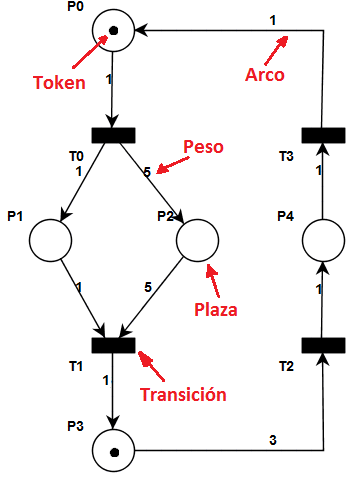
\includegraphics[width=2.3in]{./img/reddepetri.png}
		\caption{Red de Petri}
		\label{fig: petri}
	\end{figure} 

	Las Redes de Petri constan de cuatro componentes fundamentales. \textit{Fig. \ref{fig: petri}}

	\begin{itemize}
		\item \textbf{Plazas}: Las plazas de una Red de Petri, permiten representar el estado del sistema. 
     		Podr�an definirse como variables de estado que toman valores enteros (cantidad de tokens). Se representan con un c�rculo.
		\item \textbf{Transiciones}: Se grafican con un rect�ngulo. Representan el conjunto de sucesos que hacen que el estado del sistema
     		cambie.
		\item \textbf{Arcos}: Los arcos indican las conexiones entre lugares y transiciones. Nunca unen dos lugares o dos transiciones en forma
      		sucesiva. Pueden entrar o salir varios arcos de una misma transici�n o de un mismo lugar.
      		Los arcos tienen asociado un ``peso'' que indica la cantidad de tokens que se consumen o generan al atravesarlo. El disparo
      		de una transici�n retira tantos tokens de cada uno de sus lugares de entrada como lo indican los pesos de los arcos 
      		conectores y a�ade los tokens a sus lugares de salida como lo indican los pesos de los arcos de salida.
		\item \textbf{Tokens}: Los tokens representan el valor espec�fico de la condici�n o estado. Son graficados como un punto negro o un
      		n�mero natural o cero dentro de una plaza.
	\end{itemize}
	 
	\subsection{Estructura de una Red de Petri}
		Una Red de Petri Marcada queda definida como una 5-tupla de la siguiente manera:
		
		\begin{center}
			$PN = \{P, T, I^-, I^+, m_0\}$ 
		\end{center}
		
		Donde:
		\begin{itemize}
		
			\item $\boldsymbol{P = \{p_1, p_2, p_3 \ldots p_m\}}$, conjunto de $m$ lugares con $m$ finito y distinto de cero.
										
			\item $\boldsymbol{T = \{t_1, t_2, t_3 \ldots t_n\}}$, conjunto de $n$ transiciones con $n$ finito y 
				distinto de cero.
		
			\item $\boldsymbol{I}$, matriz de incidencia. Esta matriz es de dimensiones $m�n$ representa los pesos de los arcos, 
				siendo sus valores positivos cuando el arco va desde una transici�n hacia una plaza y negativos los inversos.
				As� mismo esta matriz de incidencia debe separarse en dos para representar la estructura. Estas dos matrices son:
					\begin{description}
						\item [$\boldsymbol {I-}$] Matriz de incidencia negativa. Esta matriz es de dimensiones $m�n$ representa
							los pesos de los arcos que ingresan desde los lugares de P a las transiciones de T.
						\item [$\boldsymbol {I+}$] Matriz de incidencia positiva. Esta matriz es de dimensiones $m�n$ representa
							los pesos de los arcos que salen desde las transiciones de T hacia los lugares de P. 
					\end{description}
				Para una red con ``$m$'' plazas y ``$n$'' transiciones, la matriz de incidencia es de tama�o ``$m�n$'', sus 
				elementos $a_{ij}$ son: \newline
					\begin{equation}
						\begin{matrix}
							\forall p_i \in P \wedge \forall t_j\in T \Rightarrow a_{ij}=\;
							\begin{cases} 
								\begin{matrix} 	0 		& si \; entre \; p_i \; y \; t_j\\ 
						 						  		&	 \;	no \; existen\; arcos\\
												W_{ij} 	& si \; p_i \; es \; plaza\\
													 	& de \; salida \; de \; t_j\\
												-W_{ij} & si \; p_i\; es \; plaza\\
												 		& de \; entrada \; de \; t_j 
								\end{matrix}
							\end{cases}
						\end {matrix}
						\label{eq: definicionincidencia}
					\end{equation}
				\newline
			
			\item $\boldsymbol {m_0}$ es el marcado inicial de la red, un vector de asignaci�n de tokens a las plazas de la red,
		 		de esta forma se define la configuraci�n inicial de los tokens de la red. Por ejemplo puede definirse el 
		 		marcado de una plaza como $m(i)$, esto indica la cantidad de tokens ubicados en la plaza ``$i$''.
		\end{itemize}
	
	\subsection{Ejecuci�n de una Red de Petri}
	
		El comportamiento din�mico de una red de Petri esta definido por la sensibilizaci�n y el disparo de sus transiciones
		\begin{itemize}
			\item \textbf{Transici�n sensibilizada:} Se dice que una transici�n $t_j$ esta sensibilizada si y solo si todas 
		  		las plazas de entrada a la transici�n, tienen una cantidad de tokens igual o mayor al peso indicado por el 
		  		arco que la une con la transici�n. Formalmente: \newline
			  		\begin{equation}
			  			\forall p_i \in I^-(t_j) / m(p_i) \geq W_{ij} 
			  			\label{eq: sensibilizada}
			  		\end{equation}
		  		Siendo $W_{ij}$ el peso del arco que une la plaza ``$i$" con la transici�n ``$j$".
		  
		 	 \item \textbf{Disparo de una transici�n:} El disparo de una transici�n es lo que provoca que el estado (marcado)
		  		de una Red de Petri cambie. La funci�n disparo  ($d$)   de una transici�n $t_j$  se define de la siguiente 
		  		manera. \newline
					\begin{equation}
						\begin{matrix}
							d(m_k,t_j ) \Rightarrow m_{k+1} (p_i)=\;
								\begin{cases} 
									\begin{matrix} 	m_k (p_i )-W_{ij} & \forall p_i \in I^-(t_j)\\
													m_k (p_i )+W_{ij} & \forall p_i \in I^+(t_j)\\
													m_k (p_i ) & otros\; casos 
									\end{matrix}
								\end{cases}
						\end {matrix}
						\label{eq: funciondisparo}
					\end{equation}		
				\newline
				Donde:
					\begin{description}
			  			\item [$\boldsymbol{m_k}$] es el marcado actual de la red.
			  			\item [$\boldsymbol{m_{k+1}}$] es el marcado que tomara la red luego del disparo.
			  			\item [$\boldsymbol{W_{ij}}$] son los elementos de la matriz de incidencia $I$.
					\end{description}
		\end{itemize}
		
		\subsubsection{Ecuaci�n de estado de una Red de Petri}
			La ecuaci�n de estado determina el estado de la Red de Petri a cada instante, queda definida a partir de la matriz de 
			incidencia y un vector de disparo que indica la transici�n o transiciones que deben ser disparadas. \newline
				\begin{equation}
					m_{k+1}=m_k+I�\delta_k
					\label{eq: ecuacionestado}
				\end{equation}
						
	\subsection{Arcos Inhibidores}
		En las Redes de Petri vistas anteriormente las transiciones est�n sensibilizadas cuando en las plazas de entrada existe una
		cantidad igual o mayor de tokens que el peso del arco que los une. Pero, en algunas situaciones, seria necesario que una
		transici�n se encuentre sensibilizada cuando no existan tokens en alguna de sus plazas de entrada. Para este fin existen
		los arcos inhibidores.
		Los arcos inhibidores se representan con una l�nea finalizada en un c�rculo.
		Se debe destacar que solo pueden ir desde plazas hacia las transiciones, nunca al rev�s. 
		Ahora, en una Red de Petri con Arcos Inhibidores, se dice que una transici�n esta sensibilizada cuando cumple (\ref{eq: sensibilizada}) y
		todas las plazas unidas a $t_j$ con arcos inhibidores tienen tokens.
		De esta manera la ecuaci�n de estado para una Red de Petri con arcos inhibidores toma la siguiente forma:
			\begin{equation}
				m_{k+1}=m_k+I�[\delta\; and\; !f_H(m_k,\;\delta)]
				\label{eq: ecuacionestadoH}
			\end{equation} 
		Se agrega una funci�n ``$f$'' que depende del marcado actual, del disparo a realizar y  de una funci�n ``$H$'' que determina si 
		el disparo de una transici�n esta sensibilizada o no de acuerdo a los arcos inhibidores. Esta funci�n toma solo valores ceros
		y unos, y al estar en una operaci�n ``$and$'' con el disparo, puede inhibirlo y hacer que no produzca efectos.
			\begin{equation}
				f_H (m_i,\delta)=M_{>0} (m_i)\; and\; ( H�\delta)
				\label{eq: funcionH}
			\end{equation}
		La funci�n $M_{>0}$ es una funci�n vectorial de ``$m$'' elementos. Cada componente ``$k$'' del resultado
		queda definido por (\ref{eq:Mayor})
			\begin{equation}
				\begin{matrix}
					M_{>0} (m_i)_k= \;
						\begin{cases} 
							\begin{matrix}	1 & si\;m_{ik}>0\\
											0 & si\;m_{ik}=0
							\end{matrix}
						\end{cases}
				\end {matrix} 
				\label{eq:Mayor}
			\end{equation} 


		

	
	%	REDES DE PETRI TEMPORALES
		%%%%%%%%%%%%%%%%%%%%%%%%%%%%%%%%%%%%%%%%%%%%%%%%%%%%%%%%%%%%%%%%%%%%%%%%%%%%%%%%%%%%%
%																					%
%	TRABAJO: Paper Redes de Petri con Tiempo										%
%																					%
%		Titulo: 	Ejecucion de Redes de Petri con Tiempo							%
%																					%
%		Autores:	Julian Nonino													%
%					Carlos Renzo Pisetta											%
%					Orlando Micolini												%
%																					%
%	Seccion: Redes de Petri Temporales												%	
%	Archivo: redes_de_petri_temporales.tex											%
%																					%
%%%%%%%%%%%%%%%%%%%%%%%%%%%%%%%%%%%%%%%%%%%%%%%%%%%%%%%%%%%%%%%%%%%%%%%%%%%%%%%%%%%%%
%	REVISIONES																		%
%																					%
%		19/10/2012																	%
%			Julian Nonino															%
%				Creacion de este archivo											%
%																					%
%%%%%%%%%%%%%%%%%%%%%%%%%%%%%%%%%%%%%%%%%%%%%%%%%%%%%%%%%%%%%%%%%%%%%%%%%%%%%%%%%%%%%

\section{Redes de Petri Temporales}
	
	En los modelos de Redes de Petri descriptos hasta el momento, el tiempo no estaba considerado. 
	
	En el formalismo de Redes de Petri b�sico, o aut�nomo, la abstracci�n del entorno en el que la red 
	evoluciona, incluyendo el tiempo como parte de este entorno, es total. Por lo que existe cierto 
	indeterminismo en cuanto al tiempo: no se especifica cu�ndo se disparar� una transici�n que est� 
	sensibilizada (ni si se disparar� realmente), tampoco cu�l de entre un grupo de transiciones en conflicto 
	ser� la disparada \cite{garcia_izquierdo}.
	
	Las distintas interpretaciones con tiempo de las Redes de Petri han tratado de reducir el indeterminismo 
	de distintas maneras. Entre estas interpretaciones est�n:
	\begin{enumerate}
	  	\renewcommand{\theenumi}{\Alph{enumi}}
	  	\item \underline{Redes de Petri Estoc�sticas (Stochastic Petri Net)}
	  		\\
			Se introduce una estimaci�n estoc�stica respecto del instante de disparo de una transici�n.
		\item \underline{Redes de Petri Temporizadas (Timed Petri Net)}
			\\
			Introduce una condici�n de tiempo que establece la duraci�n de la transici�n.
		\item \underline{Redes de Petri con Tiempo (Time Petri Net)}
			\\
			Introducen cotas temporales entre las cuales la transici�n puede o debe ser disparada.
	\end{enumerate}
	
	\begin{figure}[h]
		\centering
		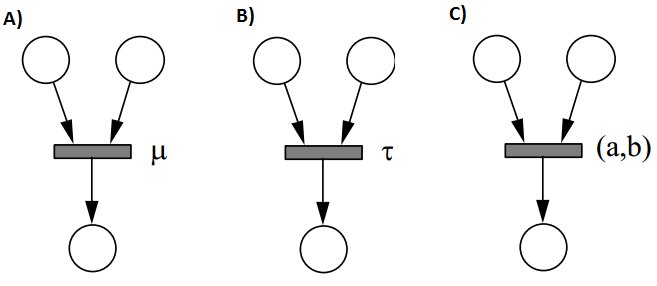
\includegraphics[width=2.5in]{./img/Petri16}
		\caption{Interpretaciones de Redes de Petri Temporales}
		\label{fig:Petri16}
	\end{figure}
	
	Existen dos maneras de interpretar el par�metro temporal asociado a una transici�n:
	\begin{itemize}
		\item Cuando el par�metro temporal determina el tiempo que ha de transcurrir desde que una transici�n 
			queda sensibilizada hasta que se dispara, procedi�ndose entonces a la retirada y colocaci�n de marcas 
			de forma at�mica, se habla de \textbf{\emph{tiempo de sensibilizaci�n (enabling time)}}.
			Est� relacionada con las \textbf{\emph{Redes de Petri con Tiempo}} (Red C de la figura \ref{fig:Petri16}).
		
		\item El par�metro temporal puede determinar tambi�n el tiempo que debe transcurrir entre la retirada 
			(instant�nea) de marcas de los lugares de entrada, y la colocaci�n (instant�nea) de marcas en los 
			lugares de salida; en este caso se habla de tiempo de \textbf{\emph{disparo (firing time)}}.
			Esto es, el disparo de la transici�n tiene tres fases (retirada de marcas de entrada, disparo, 
			colocaci�n de marcas de salida) y no es at�mico, sino que tienen una duraci�n. Por ello esta 
			interpretaci�n es tambi�n conocida como sem�ntica de duraci�n.
		 
		Est�n asociadas con las \textbf{\emph{Redes de Petri Temporizadas}} (Red B de la figura \ref{fig:Petri16}).
	\end{itemize}	
	
	%	REDES DE PETRI TEMPORALES
		%%%%%%%%%%%%%%%%%%%%%%%%%%%%%%%%%%%%%%%%%%%%%%%%%%%%%%%%%%%%%%%%%%%%%%%%%%%%%%%%%%%%%
%																					%
%	TRABAJO: Paper Redes de Petri Temporizadas										%
%																					%
%		Titulo: 	Ejecucion de Redes de Petri Temporizadas						%
%																					%
%		Autores:	Julian Nonino													%
%					Carlos Renzo Pisetta											%
%					Orlando Micolini												%
%																					%
%	Seccion: Redes de Petri Temporizadas											%	
%	Archivo: redes_petri_temporizadas.tex											%
%																					%
%%%%%%%%%%%%%%%%%%%%%%%%%%%%%%%%%%%%%%%%%%%%%%%%%%%%%%%%%%%%%%%%%%%%%%%%%%%%%%%%%%%%%
%	REVISIONES																		%
%																					%
%		19/10/2012																	%
%			Julian Nonino															%
%				Creacion de este archivo											%
%		04/04/2013																	%
%			Renzo Pisetta															%
%				Modifica															%
%																					%
%%%%%%%%%%%%%%%%%%%%%%%%%%%%%%%%%%%%%%%%%%%%%%%%%%%%%%%%%%%%%%%%%%%%%%%%%%%%%%%%%%%%%

\section{Redes de Petri Temporizadas}
			En estas redes, cada transici�n tiene asociado un par�metro $[a]$ que establece la duraci�n de la 
			transici�n, es decir la duraci�n del intervalo entre que se extraen los tokens de las plazas de 
			entrada y se colocan los tokens en las plazas de salida.
					En �sta secci�n se decribir�n las \textbf{\emph{Redes de Petri Temporizadas}} como la red \emph{B} 
		de la figura \ref{fig:Petri16}).
		
		\subsection{Definici�n matem�tica}
		
			Una \emph{Red de Petri Marcada Temporizada}, se define matem�ticamente como una 7-tupla de la siguiente 
			manera:  
			\begin{equation*}
				PN = \{P, T, I^-, I^+, H, m_0, Timer\}
			\end{equation*}
			D�nde,
			\begin{itemize}
				\item \textbf{P} es un conjunto finito y no vac�o de plazas.
				\item \textbf{T} es un conjunto finito y no vac�o de transiciones.
				\item \textbf{$I^+$} e \textbf{$I^-$} son las matrices de incidencia positiva y negativa respectivamente.
					\begin{equation*}
						P�T\rightarrow \mathbb{Z}
					\end{equation*}
				\item H es la matriz de arcos inhibidores.
					\begin{equation*}
						P�T\rightarrow\{0,1\}
					\end{equation*}
				\item $m_0$ es el marcado inicial de la red.
					\begin{equation*}
						P\rightarrow \mathbb{N}
					\end{equation*}
				\item es el conjunto de valores de duraci�n asociados a cada transici�n.
					\begin{equation*}
						T\rightarrow \mathbb{Q}^+
					\end{equation*}
			\end{itemize}
		
		El conjunto de valores \textbf{\emph{Timer}} asocia un valor racional \emph{duraci�n} a cada transici�n. De 
		manera tal que $Timer(t)=duracion$. Donde $t$ es una transici�n perteneciente a $T$.
		
		Dado que duraci�n es una referencia de tiempo, se debe cumplir que $0 \leq duracion \langle \infty$.
		
			\subsection{Estados en una Red de Petri con Tiempo}
			
			En estas Redes de Petri, el estado de la red queda definido por el vector de marcado $m$ de la 
			misma y por un vector $Intervalo$ que lleva la marca de tiempo de cada transici�n. Por lo tanto 
			el estado de una Red de Petri con Tiempo queda definido por:
			\begin{equation*}
				E = (m_0,Intervalo)
				\label{eq:estado_con_time}
			\end{equation*}
			
			Ahora, al disparar una transici�n $t$ en un instante $w_j$ produce un cambio desde el estado 
			$E = (m,Intervalo)$ a un nuevo estado $E' = (m',Intervalo')$. El nuevo marcado $m'$ se determina 
			con la ecuaci�n de estado vista anteriormente. Por otro lado, la actualizaci�n del intervalo para 
			cada transici�n $k$ sigue las siguientes reglas:
			\begin{itemize}
				\item $Intervalo'(k) = \infty$ si la transici�n $k$ no est� sensibilizada.
				\item $Intervalo'(k) = Intervalo(k) + 1$ si $k\neq t$, en el marcado $m$ esta sensibilizada 
					y sigue est�ndolo en el marcado $m'$. 
				\item $Intervalo'(k) = 0$ si $k = t$ o $k$ comienza a estar sensibilizada en el marcado $m'$.
			\end{itemize}
		
		\subsection{Regla de disparos y estados en una Red de Petri Temporizada} 
		
			En una \emph{Red de Petri Temporizada}, el disparo de una transici�n implica tres etapas.
			\begin{enumerate}
				\item Al momento que se sensibiliza la transici�n, se extrae la cantidad de tokens de las plazas 
					de entrada indicada por el arco que los une a dicha transici�n. Adem�s, se marca la transici�n
					como no sensibilizada.
					\begin{equation*}
						m_{i+1} = m_i +I^- � d
					\end{equation*}
					Se genera un nuevo estado provisorio formado a partir la extracci�n de los tokens que sensibilizaban 
					la transici�n que se esta disparando. Tambi�n, en ese instante se comienza la cuenta de tiempo.
				\item Se espera el tiempo indicado por el valor de duraci�n de la transici�n. Con la transici�n 
					marcada como desensibilizada, se espera hasta que la cuenta de tiempo, que comenz� al 
					extraerse los tokens, llegue al valor indicado por $Timer(d)$.
				\item Transcurrido el tiempo indicado por el valor de duraci�n asociado a la transici�n se colocan los tokens 
					en las plazas de salida seg�n como indican los arcos que unen a las transiciones con dichas plazas.
					\begin{equation*}
						m_{i+2} = m_{i+1} +I^+ � d
					\end{equation*}
				
			\end{enumerate}		
		\subsection{Determinaci�n de disparos posibles}
	
		Para que un disparo sea posible en una Red de Petri, debe cumplir las condiciones dadas por que todas 
		las transiciones de las cuales toma tokens tengan la cantidad necesaria de tokens, que las plazas a las 
		cuales esta conectada con arcos inhibidores no tengan tokens y que las plazas en las cuales depositan 
		tokens no superen los limites impuestos por las cotas en las plazas.
		En una Red de Petri Temporizada, al cumplirse las condiciones antes mencionadas, se dice que la transici�n 
		esta \textbf{\emph{sensibilizada}}, entonces, se ejecuta la ecuaci�n de estado de la Red de Petri utilizando 
		la matriz $I^-$. De esta manera, se remueven todos los tokens de las plazas de entrada.
			
			\begin{equation}
				m_{i+1} = m_i + I^+ � \delta
			\end{equation}

		D�nde $\delta$ es el vector de disparo que se desea ejecutar.
		A partir de dicho momento, la marca de tiempo asociada a la transici�n comienza a incrementarse seg�n su 
		vector de incrementos de tiempo. Cuando esta marca de tiempo alcanza el valor indicado por el \textbf{\emph{
		vector duraci�n}}. Cuando esto ocurre, el disparo ya esta habilitado para ser ejecutado completamente. 
		Esto se hace ejecutando la ecuaci�n de estado con la matriz de incidencia positiva, esto implica poner los tokens en 
		todas las plazas de salida.
		
			\begin{equation}
				m_{i+1} = m_i + I^- � \delta
			\end{equation}

		Durante el proceso de carga y en el instante en el cual este termina, las marcas de tiempo de todas las 
		transiciones valen cero. 
		Luego, a cada ciclo de reloj, si la transici�n se sensibiliz� y logo ejecutar la primera etapa del disparo, 
		la marca de tiempo se incrementa la cantidad de unidades que indica el \textbf{\emph{vector de incrementos de marcas 
		de tiempo}}.
		La marca de tiempo vuelve a cero solo cuando la transici�n completa ambas fases de su disparo.


	%	IP core
		%%%%%%%%%%%%%%%%%%%%%%%%%%%%%%%%%%%%%%%%%%%%%%%%%%%%%%%%%%%%%%%%%%%%%%%%%%%%%%%%%%%%%
%																					%
%	TRABAJO: Paper Redes de Petri Temporizadas										%
%																					%
%		Titulo: 	Ejecucion de Redes de Petri Temporizadas						%
%																					%
%		Autores:	Julian Nonino													%
%					Carlos Renzo Pisetta											%
%					Orlando Micolini												%
%																					%
%	Seccion: IP core																%	
%	Archivo: ip_core.tex															%
%																					%
%%%%%%%%%%%%%%%%%%%%%%%%%%%%%%%%%%%%%%%%%%%%%%%%%%%%%%%%%%%%%%%%%%%%%%%%%%%%%%%%%%%%%
%	REVISIONES																		%
%																					%
%		19/10/2012																	%
%			Julian Nonino															%
%				Creacion de este archivo											%
%																					%
%%%%%%%%%%%%%%%%%%%%%%%%%%%%%%%%%%%%%%%%%%%%%%%%%%%%%%%%%%%%%%%%%%%%%%%%%%%%%%%%%%%%%
\section{IP cores}

		La arquitectura de este IP core se mantiene en su mayor parte igual a la de las versiones anteriores. 
		Con respecto a la versi�n que procesa \emph{Redes de Petri con Tiempo}, se quitaron los vectores \emph{EFT} 
		y \emph{LFT}, en su lugar se agreg� el \textbf{\emph{vector duraci�n}}. Se mantuvo el \textbf{\emph{vector de 
		incrementos de tiempo}} y el \textbf{\emph{vector de tiempo de sensibilizaci�n}}.
		 
		\subsection{Estructuras de datos para Redes de Petri Temporizadas}
	
		Como se muestra en la figura \ref{fig:diseno48} las estructuras de datos necesarias para la resoluci�n 
		de Redes de Petri Temporizadas son tres:
		\begin{itemize}
		  	\item Vector \textbf{\emph{duraci�n}}.
		  	\item Vector de \textbf{\emph{marcas temporales}}.
		  	\item Vector de \textbf{\emph{escala de incrementos de tiempo}}.
		\end{itemize}
		
		\begin{figure*}[!b]
			\centering
			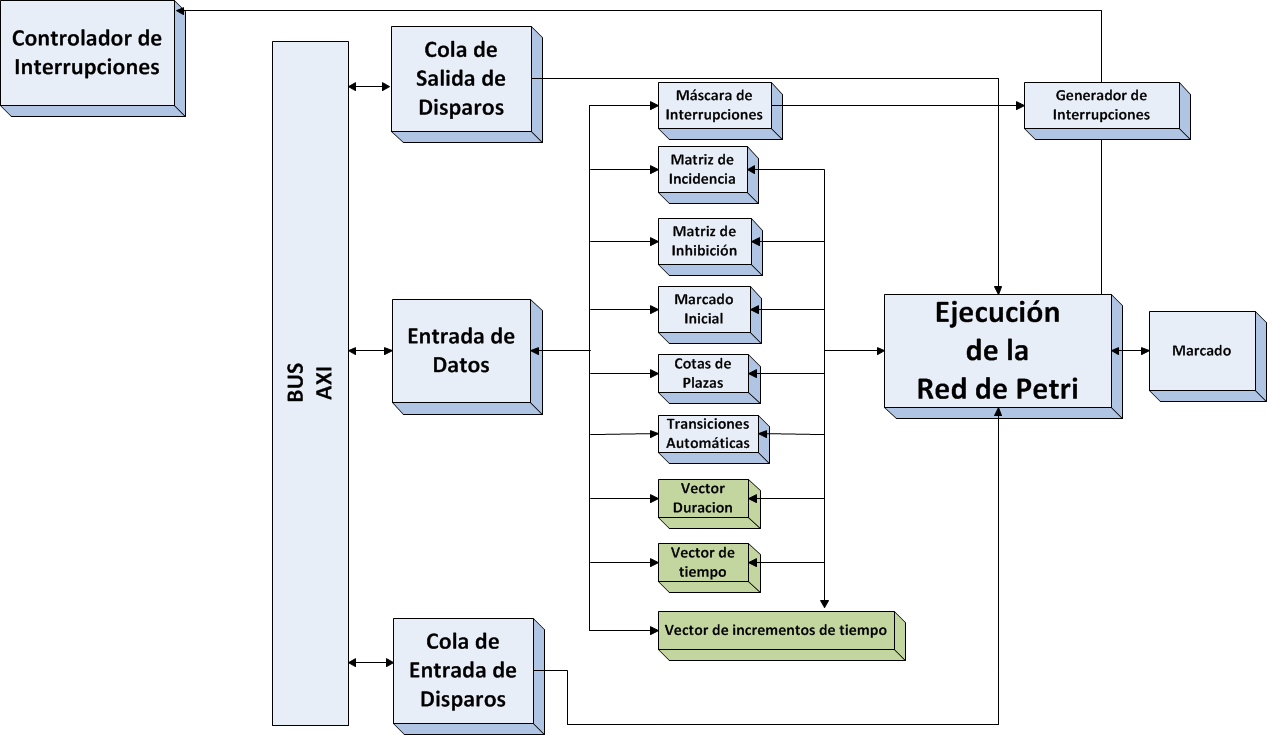
\includegraphics[width=6.5in]{./img/diseno48}
			\caption{Arquitectura del procesador de Redes de Petri Temporizadas}
			\label{fig:diseno48}
		\end{figure*}
		
		Los cuatro vectores tienen como cantidad de elementos el n�mero de transiciones. Los dos primeros son 
		tiene un tama�o de elementos parametrizable pero por defecto tienen 32 bits. El vector de escala de 
		incrementos de tiempo, por defecto toma el un tama�o de elementos de 5 bits.

		\subsection{Algoritmo de Ejecuci�n con Redes de Petri Temporizada}
	Basados en la teoria descripta se creo un algoritmo de ejecuci�n de disparos en una red de petri que se describe a continuaci�n es sintetizable en hardware y requiere 
	�nicamente 2 ciclos de reloj para ejecutar todos los pasos y a la vez permita un dise�o parametrizable en cuanto al tama�o y cantidad de elementos que soporte.

	\begin{enumerate}
		\item Espera de disparo en Cola de entrada de disparos.
		\item Llegado el disparo se calcula un vector binario de longitud cantidad de transiciones con un �nico 1 en el lugar correspondiente al n�mero de disparo, en funci�n del n�mero de transici�n que contenga. Este vector se utiliza para incrementar los contadores de disparos.
			Son considerados disparos en espera.
		\item Se calcula todos los posibles resultados para todos los disparos, hayan sido pedidos o no para confeccionar una matriz resultado donde cada columna Ci representa el nuevo marcado si la transici�n Ti  se disparara.
		\item Se crea una matriz de signos auxiliar con los signos correspondientes a cada elemento de la matriz resultado. 
		\item Se crea una matriz de inhibici�n auxiliar en funci�n del marcado actual y la Matriz de Inhibici�n determinando las plazas con arcos inhibidores que tienen tokens.
		\item Se crea una matriz de cotas en funci�n de la matriz resultados y las cotas de las plazas determinando cual fue superada para cada plaza por cada posible resultado
		\item Se crea un vector en el cual cada elemento corresponde a una columna de la matriz de signos y determina si esa transici�n es o no posible en funci�n si alg�n elemento de su resultado es negativo.
		\item Se crea un vector en el cual cada elemento corresponde a una columna de la matriz de inhibici�n y determina las transiciones que no pueden ser disparada debido a arcos inhibidores.
		\item Se crea un vector en el cual cada elemento corresponde a una columna de la matriz de cotas el cual determina que transiciones no pueden ser disparadas debido a que provocar�an superar las cotas de las plazas.
		\item En funci�n de los vectores creados en los puntos 7, 8 y 9 se crea un vector que determina las transiciones sensibilizadas. 
		\item Para determinar las transiciones a disparar se unen los disparos pendientes y las transiciones autom�ticas. Luego en funci�n de los disparos posibles y que la cola de disparos de salida no est� llena se actualiza el marcado �nicamente retirando tokens de las plazas  de entrada en funci�n de la matriz I-.
		\item Se habilita contador de transici�n temporizada.
		\item En cada clock de reloj se actualiza el vector de tiempo (contador saturado) de cada transici�n sensibilizada increment�ndolo seg�n el vector de incremento de tiempo correspondiente a partir de que la transici�n es disparada.
		\item Cuando el vector de tiempo supera la duraci�n de la transici�n se completa el disparo actualizando el marcado �nicamente agregando los tokens en las plazas de salida en funci�n de la matriz I+.
		\item Se incrementa contador de cola de salida correspondiente a transici�n ejecutada.
	\end{enumerate}	
	
	%	Analisis de Rendimiento
		%%%%%%%%%%%%%%%%%%%%%%%%%%%%%%%%%%%%%%%%%%%%%%%%%%%%%%%%%%%%%%%%%%%%%%%%%%%%%%%%%%%%%
%																					%
%	TRABAJO: Paper Mejoras en el procesador de Redes de Petri						%
%																					%
%		Titulo: 	Soft Core parametrizable con procesamiento de Redes de Petri	%
%																					%
%		Autores:	Julian Nonino													%
%					Carlos Renzo Pisetta											%
%					Orlando Micolini												%
%																					%
%	Seccion: ANALSIS DE RENDIMIENTO													%	
%	Archivo: analisis_rendimiento.tex												%
%																					%
%%%%%%%%%%%%%%%%%%%%%%%%%%%%%%%%%%%%%%%%%%%%%%%%%%%%%%%%%%%%%%%%%%%%%%%%%%%%%%%%%%%%%

 \section{An�lisis de Rendimiento}
 		Una vez terminado el IP Core para comprobar su correcto funcionamiento y ver si �ste realmente 
 		tiene una mejora en los tiempos de sincronizaci�n, se realizaron mediciones para distinto n�mero
 		de iteraciones, tanto para el Procesador de Petro como para Sem�foros. La elecci�n de este segundo
 		m�todo de sincronizaci�n se basa en que son el mecanismo m�s ligero para realziar �stas tareas.
 		A partir de estas mediciones se realiz� la gr�fica de la Figura \ref{fig:resultados13} 
 		
		\begin{figure}[h]
			\centering
			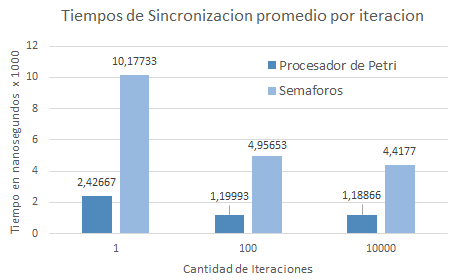
\includegraphics[width=3in]{resultados13}
			\caption{Tiempos de sincronizaci�n procesador de Redes de Petri vs. Sem�foros}
			\label{fig:resultados13}
		\end{figure}		
		
		Se puede observar que, para todos los casos, el procesador de Petri es aproximadamente cuatro veces
		m�s rapido que los Sem�foros.
		
	%	CRECIMIENTO DEL IP CORE
		%%%%%%%%%%%%%%%%%%%%%%%%%%%%%%%%%%%%%%%%%%%%%%%%%%%%%%%%%%%%%%%%%%%%%%%%%%%%%%%%%%%%%
%																					%
%	TRABAJO: Paper Mejoras en el procesador de Redes de Petri						%
%																					%
%		Titulo: 	Soft Core parametrizable con procesamiento de Redes de Petri	%
%																					%
%		Autores:	Julian Nonino													%
%					Carlos Renzo Pisetta											%
%					Orlando Micolini												%
%																					%
%	Seccion: CRECIMIENTO DEL IP CORE												%	
%	Archivo: crecimiento_ip_core.tex												%
%																					%
%%%%%%%%%%%%%%%%%%%%%%%%%%%%%%%%%%%%%%%%%%%%%%%%%%%%%%%%%%%%%%%%%%%%%%%%%%%%%%%%%%%%%

\section{Crecimiento del IP Core}
		Una vez visto el correcto funcionamiento del IP Core, se evalu� el crecimiento del procesador 
		en funci�n de los par�metros que posee. Para esto se generaron procesadores de 8x8, 16x16 y 
		32x32, con capacidad de 7 bits por plaza y se graficaron los valores que se pueden 
		observar en la Figura \ref{fig:resultados05}.
		\begin{figure}[h]
			\centering
			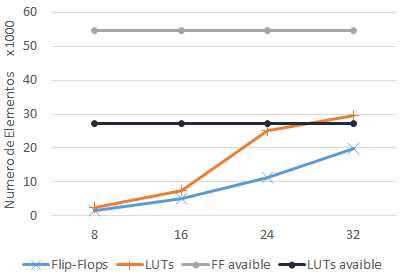
\includegraphics[width=3in]{resultados08}
			\caption{Diferentes implementaciones del procesador de Redes de Petri}
			\label{fig:resultados05}
		\end{figure}
	
		Es posible ver que el crecimiento del IP Core no es algo para despreciar, puesto que 
		se incrementa r�pidamente a medida que aumentamos el tama�o de elementos soportados.
		Se observa tambi�n que si bien la pendiente aumenta, �stos incrementos son cada vez menores,
		tendiendo a linealizar para los IP Cores m�s grandes.
		
		Tambien podemos observar los elementos disponibles que tenemos en una determinada FPGA, para este
		caso una Spartan6 de Xilinx. Vemos que desarrollar una implementacion de 32x32 es inalcansable, en este
		caso es necesario pasar a una con mas recursos. 
		
			
	%	CONCLUSION
		\section{Conclusion and Contributions}

	In this paper, a Time Petri Processor is developed, which decouples the concurrency from sequential 
	processing, it has the following particularities:
	\begin{itemize}
  		\item On tasks, where measurements have been done, the processor allows synchronization of 
  				threads, with improvements up to 70\%.
		\item There is a direct relationship between the graph and the processor program, since this 
				is programmed with the state equation's matrixes and vectors.
		\item Multiple are admitted shots simultaneously in the same transition.
		\item Allows programming priorities since the shots are solved in parallel and are selected 
				according to priorities module.
		\item Decides if the shot can be executed or not in 2 clock cycles.
		\item The system programming is easier to do, since the processes are decoupled from the concurrency.
		\item This processor can be programmed at run time, thus it is possible to decrease the size 
				of the matrix in hardware by using spatial and temporal locality.
	\end{itemize}
	
	The difficulty of this implementation is because of the growth of the resources needed by the 
	increase of places and transitions. This implies that is difficult to implement a system for 
	dimensions greater than 32x32 in ZedBoard, to mitigate this difficulty new designs have been 
	proposed and are being worked on, these are: Petri Net Processor with pipeline architecture and 
	support for Hierarchical Petri Nets.

	%	APENDICES
		%%%%%%%%%%%%%%%%%%%%%%%%%%%%%%%%%%%%%%%%%%%%%%%%%%%%%%%%%%%%%%%%%%%%%%%%%%%%%%%%%%%%%
%																					%
%	TRABAJO: Paper Mejoras en el procesador de Redes de Petri						%
%																					%
%		Titulo: 	Soft Core parametrizable con procesamiento de Redes de Petri	%
%																					%
%		Autores:	Julian Nonino													%
%					Carlos Renzo Pisetta											%
%					Orlando Micolini												%
%																					%
%	Seccion: Apendices																%	
%	Archivo: apendices.tex															%
%																					%
%%%%%%%%%%%%%%%%%%%%%%%%%%%%%%%%%%%%%%%%%%%%%%%%%%%%%%%%%%%%%%%%%%%%%%%%%%%%%%%%%%%%%

% if have a single appendix:
%\appendix[Proof of the Zonklar Equations]
% or
%\appendix  % for no appendix heading
% do not use \section anymore after \appendix, only \section*
% is possibly needed

% use appendices with more than one appendix
% then use \section to start each appendix
% you must declare a \section before using any
% \subsection or using \label (\appendices by itself
% starts a section numbered zero.)
%


\appendices
\section{Proof of the First Zonklar Equation}
Appendix one text goes here.

% you can choose not to have a title for an appendix
% if you want by leaving the argument blank
\section{}
Appendix two text goes here.

	%	AGRADECIMIENTOS
		%%%%%%%%%%%%%%%%%%%%%%%%%%%%%%%%%%%%%%%%%%%%%%%%%%%%%%%%%%%%%%%%%%%%%%%%%%%%%%%%%%%%%
%																					%
%	TRABAJO: Paper Mejoras en el procesador de Redes de Petri						%
%																					%
%		Titulo: 	Soft Core parametrizable con procesamiento de Redes de Petri	%
%																					%
%		Autores:	Julian Nonino													%
%					Carlos Renzo Pisetta											%
%					Orlando Micolini												%
%																					%
%	Seccion: Agradecimientos														%	
%	Archivo: agrademientos.tex														%
%																					%
%%%%%%%%%%%%%%%%%%%%%%%%%%%%%%%%%%%%%%%%%%%%%%%%%%%%%%%%%%%%%%%%%%%%%%%%%%%%%%%%%%%%%
		
	% use section* for acknowledgement
	\section*{Acknowledgment}
		The authors would like to thank...

	%	REFERENCIAS
		% Can use something like this to put references on a page
		% by themselves when using endfloat and the captionsoff option.
		\ifCLASSOPTIONcaptionsoff
  			\newpage
		\fi
		% trigger a \newpage just before the given reference number - used to balance the columns on the last page
		% adjust value as needed - may need to be readjusted if the document is modified later
		%\IEEEtriggeratref{8}
		% The "triggered" command can be changed if desired:
		%\IEEEtriggercmd{\enlargethispage{-5in}}
	
		% references section
		
		% can use a bibliography generated by BibTeX as a .bbl file BibTeX documentation can be easily obtained at:
		% http://www.ctan.org/tex-archive/biblio/bibtex/contrib/doc/
		% The IEEEtran BibTeX style support page is at:
		% http://www.michaelshell.org/tex/ieeetran/bibtex/
			\bibliographystyle{IEEEtran}
			% argument is your BibTeX string definitions and bibliography database(s)
			\bibliography{./bib/referencias}
		%\bibitem{PaperProcesador}{Micolini, Orlando; Pereyra, Martan M.; Gallia, Nicolas A.; Alasia, Melisa A. Sistema Multi-Core 
		%Heterogeneo, sincronizado por un Procesador de Petri sobre FPGA.}

	%	BIOGRAFIAS
		%%%%%%%%%%%%%%%%%%%%%%%%%%%%%%%%%%%%%%%%%%%%%%%%%%%%%%%%%%%%%%%%%%%%%%%%%%%%%%%%%%%%%
%																					%
%	TRABAJO: Paper Redes de Petri Temporizadas										%
%																					%
%		Titulo: 	Ejecucion de Redes de Petri Temporizadas						%
%																					%
%		Autores:	Julian Nonino													%
%					Carlos Renzo Pisetta											%
%					Orlando Micolini												%
%																					%
%	Seccion: Biografias																%	
%	Archivo: biografias.tex															%
%																					%
%%%%%%%%%%%%%%%%%%%%%%%%%%%%%%%%%%%%%%%%%%%%%%%%%%%%%%%%%%%%%%%%%%%%%%%%%%%%%%%%%%%%%
%	REVISIONES																		%
%																					%
%		18/10/2012																	%
%			Julian Nonino															%
%				Creacion de este archivo											%
%		18/10/2012																	%
%			Renzo Pisetta															%	
%				Codificacion de esta seccion										%
%		04/04/2013																	%
%			Julian Nonino															%
%				Actualizacion 														%		
%																					%
%%%%%%%%%%%%%%%%%%%%%%%%%%%%%%%%%%%%%%%%%%%%%%%%%%%%%%%%%%%%%%%%%%%%%%%%%%%%%%%%%%%%%

% biography section
% 
% If you have an EPS/PDF photo (graphicx package needed) extra braces are
% needed around the contents of the optional argument to biography to prevent
% the LaTeX parser from getting confused when it sees the complicated
% \includegraphics command within an optional argument. (You could create
% your own custom macro containing the \includegraphics command to make things
% simpler here.)
%\begin{biography}[{\includegraphics[width=1in,height=1.25in,clip,keepaspectratio]{./jnonino.png}}]{Juli�n Nonino}
% or if you just want to reserve a space for a photo:


\begin{IEEEbiography}[{\includegraphics[width=1in,height=1.25in,clip,keepaspectratio]{./img/jnonino.png}}]{Juli�n Nonino}
(M'2011) naci� en Rio Cuarto, C�rdoba, Argentina el d�a 16 de octubre de 1988. En el a�o 2012 obtuvo 
el t�tulo de grado Ingeniero en Computaci�n de la Facultad de Ciencias Exactas, F�sicas y Naturales 
de la Universidad Nacional de C�rdoba.
Actualmente se desempe�a como Ingeniero de Software en Motorola Mobility of Argentina S.A. 
En el ambito universitario, precisamente en la Facultad de Ciencias Exactas, F�sicas y Naturales de 
la Universidad Nacional de C�rdoba, colabora en las c�tedras Ingenier�a de Software y Gesti�n de la 
Calidad de Software. Tambi�n, en el Laboratorio de Arquitectura de Computadoras de la misma universidad, 
realiza actividades relacionadas con el dise�o e implementaci�n de software y hardware optimizado 
para sistemas de computaci�n en paralelo basados en Redes de Petri.
\end{IEEEbiography}

\begin{IEEEbiography}[{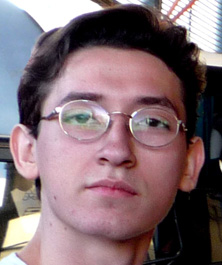
\includegraphics[width=1in,height=1.25in,clip,keepaspectratio]{./img/crpisetta}}]{Carlos Renzo Pisetta}
(M'2011) naci� en C�rdoba, Argentina el d�a 07 de junio de 1989. En el a�o 2012 obtuvo 
el t�tulo de grado Ingeniero en Computaci�n de la Facultad de Ciencias Exactas, F�sicas y Naturales 
de la Universidad Nacional de C�rdoba.
Actualmente se desempe�a como investigador en el Laboratorio de Arquitectura de Computadoras en la UNC(FCEFyN) abocado 
al dise�o e implementaci�n de software y hardware optimizado para sistemas de computaci�n en paralelo basados en Redes de Petri.
\end{IEEEbiography}

\begin{IEEEbiography}[{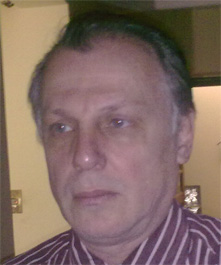
\includegraphics[width=1in,height=1.25in,clip,keepaspectratio]{./img/omicolini}}]{Orlando Micolini}
Grado en Ingeniero Electricista Electr�nico, a�o 1981, de la UNC (FCEFyN) Argentina. Postgrado Especialista en Telecomunicaciones,
a�o 2002, de la UNC (FCEFyN) Argentina. Mag�ster en Ciencias de la Ingenier�a, a�o 2002, de la UNC (FCEFyN) Argentina.
Director de SCS S.R.L, desde 1991 a 2008. Director de la Carrera de Ingenier�a en Computaci�n en la  UNC (FCEFyN) Argentina
(2004-actualidad). Titular de la asignatura Arquitectura de Computadoras en la  UNC (FCEFyN) Argentina (1996-actualidad). 
Actualmente est� trabajando, realizando el doctorado de Ciencias Inform�tica en la Universidad Nacional de la Plata, 
en sistemas multi-core heterog�neos con Redes de Petri.
\end{IEEEbiography}

% You can push biographies down or up by placing
% a \vfill before or after them. The appropriate
% use of \vfill depends on what kind of text is
% on the last page and whether or not the columns
% are being equalized.
%	\vfill
	
% Can be used to pull up biographies so that the bottom of the last one
% is flush with the other column.
%\enlargethispage{-5in}

%	FIN DEL DOCUMENTO
	\end{document}
